\chapter{Related Work} \label{chap:Chapter2}       
\epigraph{``This is where technology is now, imagine where we can go in the future” }{\textit{Timothy Chung}}

Σε αυτό το \emph{Chapter} περιγράφονται τρόποι - από την βιβλιογραφία - με τους οποί\-ους, υπάρχουσες εφαρμογές 
μεμονωμένων \hyperref[abbr:UAV]{UAV}, καθώς και drone swarms επιλύουν το localization pro\-blem. Κάποια από τα συστήματα στις παρακάτω έρευνες έχουν καθαρά
θεωρητική πλευρά, ενώ άλλα έχουν δοκιμαστεί σε real-life scenarios.
Τέλος, σε αρκετές από αυτές τις εφαρμογές χρησιμοποιούνται τεχνικές που θα αναλυθούν στο \emph{Chapter} \ref{chap:Chapter3} 
σε μεγαλύτερο βάθος, καθώς θα αποτελέσουν το προαπαιτούμενο θεωρητικό και μαθηματικό υπόβαθρο για τον σχεδιασμό του συστήματος της παρούσας διπλωματικής.

% Κυρίως, αυτά που θα μελετήσουμε θα αφορούν Cooperative Localization (\hyperref[abbr:CL]{CL}) των \hyperref[abbr:UAV]{UAV}s, ενώ επίσης
% μας ενδιαφέρουν τα Distributed Computation - Real Time Location System (\hyperref[abbr:RTLS]{RTLS}) \cite{rtls}. 

Το πρόβλημα του Local Positioning System 
(\hyperref[abbr:LPS]{LPS}) \cite{lps} έχει ερευνηθεί από διάφορες οπτικές\udot οι οποίες μπορεί να βασίζονται σε 
\hyperref[abbr:RF]{RF}, sound waves ή ακόμα και να είναι image oriented.

Σχεδόν βέβαιο είναι επίσης, ότι από όποια κατεύθυνση και αν προσεγγίσουμε το \hyperref[abbr:LPS]{LPS} να έχουμε την ανάγκη να 
χρησιμοποιήσουμε κάποια τεχνική για να συνενώσουμε όλες τις πληροφορίες που έχουμε από τους διάφορους αισθητήρες για κάθε μεμονωμένο 
time-frame - με δεδομένο ότι κάνουμε χρήση πολλαπλών αισθητήρων ώστε να μειώσουμε την εντροπία, συνεπώς και την αβεβαιότητα ως 
προς την εκτίμηση της θέσης. 
Την ανάγκη αυτού έρχεται να καλύψει η έννοια του \emph{sensor fusion} \cite{sensor-fusion}. Όπως επίσης, συχνά 
έχουμε την ανάγκη φιλτραρίσματος των μετρήσεων - που οδηγεί σε καλύτερα αποτελέσματα - με μερικούς γνωστούς 
αλγόριθμους που να το επιτυγχάνουν - να είναι το  
Extended Kalman Filter (\hyperref[abbr:EKF]{EKF}), Unscented Kalman Filter (\hyperref[abbr:UKF]{UKF}), Covariance Intersection  
Filter (\hyperref[abbr:CIF]{CIF}),  Split  Covariance  Intersection  Filter (\hyperref[abbr:SCIF]{SCIF}) και  Belief  Propagation 
(\hyperref[abbr:BP]{BP}) \cite{fusion-filters}. 

% Τέλος, είναι επίσης σημαντικό να αναφερθούν τα βασικά \emph{coordinate frames} τα οποία χρησιμοποιούνται. 
% Αισθητήρες όπως το \hyperref[abbr:IMU]{IMU} και το compass κάνουνε μετρήσεις με γνώμονα το ίδιο το σώμα 
% του αντικειμένου για αυτό - σε αυτήν την περίπτωση το σύστημα αξόνων ονομάζεται body frame (B frame) \cite{uwb-imu-gps1}.
% Συχνά είναι όμως βολικό να μετατρέψουμε αυτές τις μετρήσεις σε ένα κοινό North East Down (\hyperref[abbr:NED]{NED}) 
% σύστημα, οπότε τότε αναφερόμαστε σε N frame \cite{uwb-imu-gps1} \cite{body-frames}. Παράδειγμα μεταξύ των δύο 
% συστημάτων βρίσκεται στο \emph{Figure} \ref{fig:Important-coordinate-frames}.

% \begin{figure} [H]
% 	\centering
% 	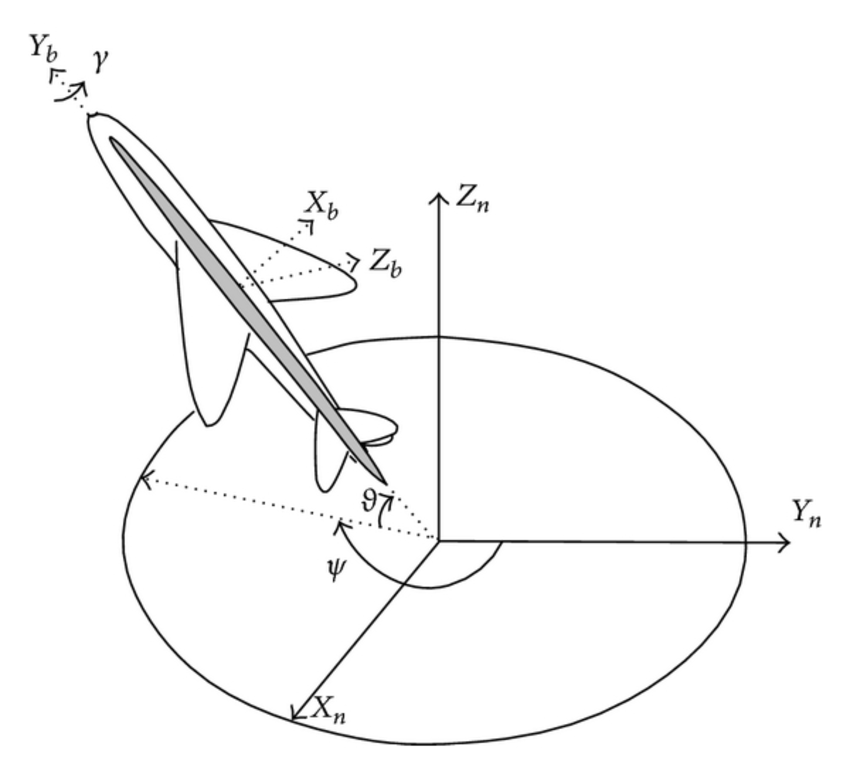
\includegraphics[width=0.6\linewidth]{Images/Related-Work/b-frame-n-frame-and-Euler-angles.png}
% 	\decoRule
% 	\caption[Important coordinate frames]{Important coordinate frames \cite{body-frames}}
% 	\label{fig:Important-coordinate-frames}
% \end{figure}


% ------------------------------------------------------------------------------------
\section{Radio Frequency}
Το πιο εύκολο που μπορούμε να φανταστούμε είναι να χρησιμοποιήσουμε \hyperref[abbr:RF]{RF} τε\-χνο\-λο\-γίες
όπως WiFi, Zigbee και Ultra-Wideband (\hyperref[abbr:UWB]{UWB}) για την επικοινωνία και την υλοποίηση του \hyperref[abbr:LPS]{LPS}.   
Το WiFi είναι εύκολα προσβάσιμο\udot με μικρό κόστος ενώ το Zigbee προτιμάται για
low power consumption εφαρμογές. Όμως προβλήματα αυτών των δύο είναι, ότι το 
WiFi έχει μικρή εμβέλεια\footnote{Αυτό είναι κυρίως πρόβλημα για outdoor scenarios} όπως επίσης είναι πολύ εύκολο 
να υπάρχουν παρεμβολές από τις υπόλοιπες γειτονικές συσκευές\footnote{Αυτό είναι κυρίως πρόβλημα για indoor scenarios} 
άρα δεν το καθιστά καλή λύση για swarms. Το Zigbee επιλύει κάποια από αυτά τα 
προβλήματα\footnote{Σε indoor σενάρια παραμένει η δυσκολία για collision-free formation}. Συχνότερη εφαρμογή έχουν 
τα \hyperref[abbr:UWB]{UWB} καθώς επιλύει θέματα σχετικά με την ακρίβεια των μετρήσεων, το κόστος καθώς και την 
εμβέλεια\udot ταυτόχρονα \cite{uwb-imu-gps3}. Τέλος, με την χρήση του \hyperref[abbr:UWB]{UWB} επίσης, μπορούμε εύκολα να δημιουργήσουμε
ένα Flying Ad-hoc Network (\hyperref[abbr:FANET]{FANET}) το οποίο βοηθάει στην ευελιξία του συστήματος.


% ---------------------
\subsection{WiFi}
Μία αρχική προσέγγιση \cite{wifi-passive-active-drone-localization}

\begin{figure} [H]
	\centering
    % -----------------
		\begin{minipage}{.48\textwidth}
			\centering
			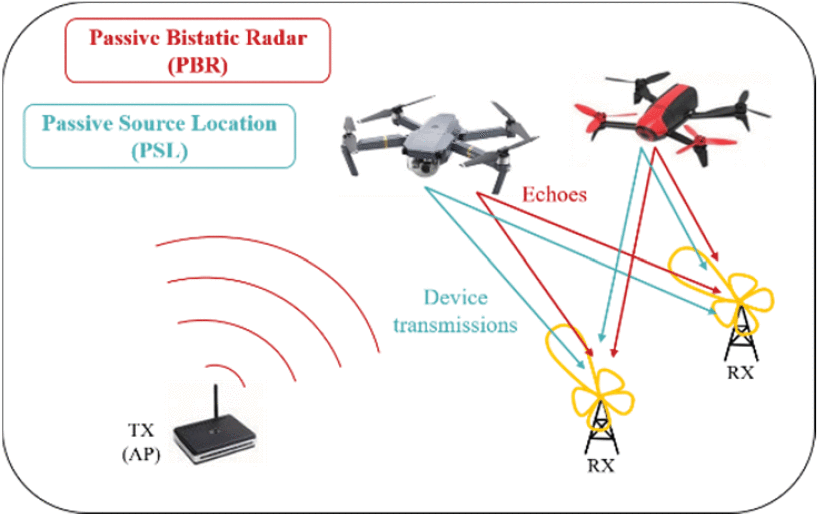
\includegraphics[width=\linewidth]{Images/Related-Work/PBR-and-PSL-approaches.png}
			{(a) PBR and PSL (\href{https://ieeexplore.ieee.org/document/9253794/figures#figures}{URL})}
		\end{minipage}%
		\hspace*{+1cm}
		% -----------------
		\begin{minipage}{.48\textwidth}
			\centering
			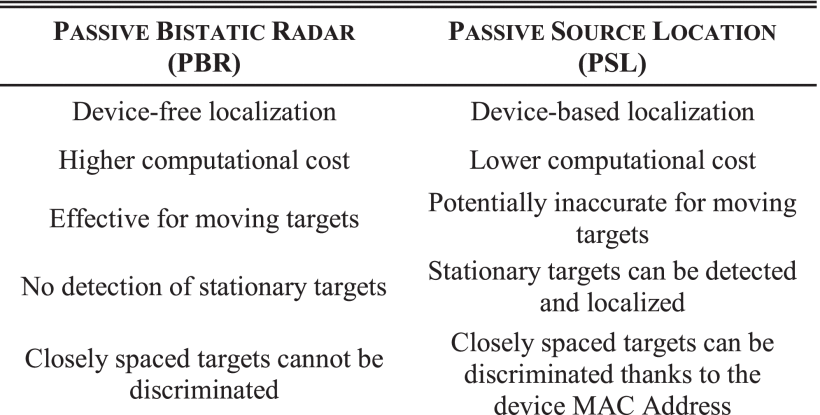
\includegraphics[width=\linewidth]{Images/Related-Work/PBR-and-PSL-Features.png}
			{(b) PBR and PSL Features (\href{https://ieeexplore.ieee.org/document/9253794/figures#figures}{URL})}
		\end{minipage}
	% -----------------
    \hfill \break
    \decoRule
    \caption[PBR and PSL localization Appoaches]{PBR and PSL localization Appoaches based on \cite{wifi-passive-active-drone-localization}}
    \label{fig:[PBR-and-PSL]}
\end{figure}

% ---------------------

% \subsection{UWB, IMU and GPS}
% Στο \cite{uwb-imu-gps1} θεωρείται ότι υπάρχουν Ν αριθμημένα \hyperref[abbr:UAV]{UAV}, τα οποία επικοινωνούν σε \hyperref[abbr:UWB]{UWB}, 
% αξιοποιώντας την λογική του γράφου - για την αναπαράσταση τους - όπως 
% περιγράφτηκε στο \emph{Section} \ref{sec:Chapter3-3}. Ενώ κάθε node περιλαμβάνει \hyperref[abbr:IMU]{IMU}, Compass, \hyperref[abbr:GPS]{GPS} και A\-lti\-tu\-de and Heading Re\-fe\-re\-nce 
% System (\hyperref[abbr:AHRS]{AHRS})\footnote{Αξιοποιείται από ένα flight control unit} με την χρήση των οποίων μπορούν σε N frame να συλλέξουν 
% πληροφορίες όπως παρουσιάζονται στους πα\-ρα\-κά\-τω πίνακες για κάθε time-frame k.

% \begin{gather*}
% 	\textbf{GPS Position:}\quad r^k_{i, GPS} = \left[x^k_{i, GPS} \quad y^k_{i, GPS} \quad z^k_{i, GPS}\right]^T \\
% 	\textbf{Velocity estimation:}\quad\hat{v}^k_i = \left[\hat{v}^k_{xi} \quad \hat{v}^k_{yi} \quad \hat{v}^k_{zi}\right]^T \\
% 	\textbf{Acceleration estimation:}\quad\hat{a}^k_i = \left[\hat{a}^k_{xi} \quad \hat{a}^k_{yi} \quad \hat{a}^k_{zi}\right]^T
% \end{gather*}

% Σε αυτό το \hyperref[abbr:UWB]{UWB} δίκτυο είναι εύκολο το κάθε drone να μετρήσει την απόσταση του από ένα γειτονικό
% μέσω \hyperref[abbr:ToA]{ToA}-based \hyperref[abbr:RTT]{RTT} μεθόδου, με όνομα Single-sided Two-way Ranging (\hyperref[abbr:SS-TWR]{SS-TWR}),
% όπως περιγράφει η εξίσωση (\ref{eq:ss-twr}). Τα $T_{round}$ και $T_{reply}$ είναι
% οι χρόνοι που μετρήθηκαν για την εκτίμηση απόστασης - η οποία όμως περιλαμβάνει σφάλμα ως εξής, $\norm{r_i - r_j}$ η πραγματική απόσταση και $n_{UWB}$ τυχαία μεταβλητή με τυπική απόκλιση ίση με 
% $0.1m$\footnote{Βάση θεώρησης των συγγραφών της έρευνας} και στο \emph{Figure} \ref{fig:SS-TWR} υπάρχει παράδειγμα αυτής.

% \begin{gather}
%     d_{ij} = \frac{1}{2}(T_{round} - T_{reply}) \times c = \norm{r_i - r_j} + n_{UWB}, \quad with \quad n_{UWB} \sim N(0, \sigma^2_{UWB}) \label{eq:ss-twr}
% \end{gather}

% \begin{figure} [H]
% 	\centering
% 	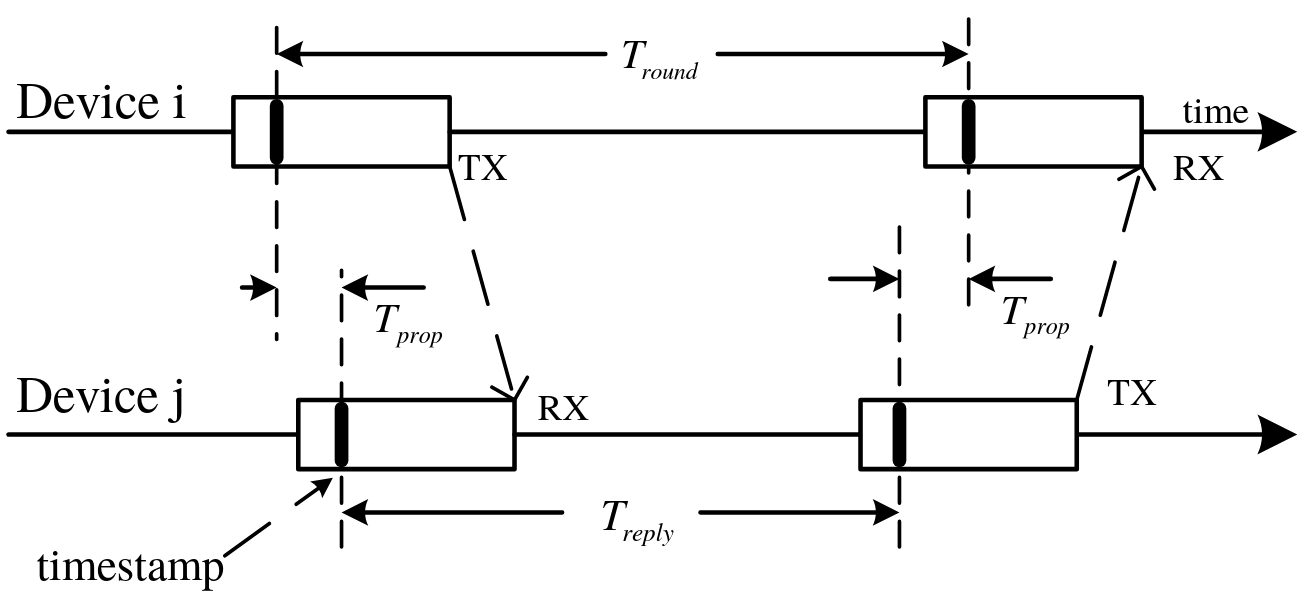
\includegraphics[width=0.69
% 	\linewidth]{Images/Related-Work/Single-Sided-Two-Way-Ranging-SS-TWR-5.png}
% 	\decoRule
% 	\caption[Illustration of Single-sided Two-way ranging]{Illustration of Single-sided Two-way ranging \cite{uwb-imu-gps1}}
% 	\label{fig:SS-TWR}
% \end{figure}

% Παρόμοιας λογικής σφάλματα θεωρείται ότι συμπεριλαμβάνουν και οι μετρήσεις από
% τους άλλους αισθητήρες, ενώ επίσης ότι το κάθε node μπορεί να μεταφέρει τις πληροφορίες 
% αυτές στα υπόλοιπα.

% Πριν το relative position estimation, για λόγους που έχουν να κάνουν με 
% Ranging outlier rejection και Ranging failure data completion γίνεται ένα 
% preprocessing με χρήση του \hyperref[abbr:EKF]{EKF} στα δεδομένα - όπως 
% παρουσιάζεται στο \emph{Figure} \ref{fig:Data-preprocessing-work-flow-using-EKF} -
% ώστε να έχουμε σαν αποτέλεσμα μετά από αυτό το στάδιο μία καλύτερη εκτίμηση των αποστάσεων $d_{ij}$ 
% για κάθε \emph{i} και \emph{j} nodes. 

% \begin{figure} [H]
% 	\centering
% 	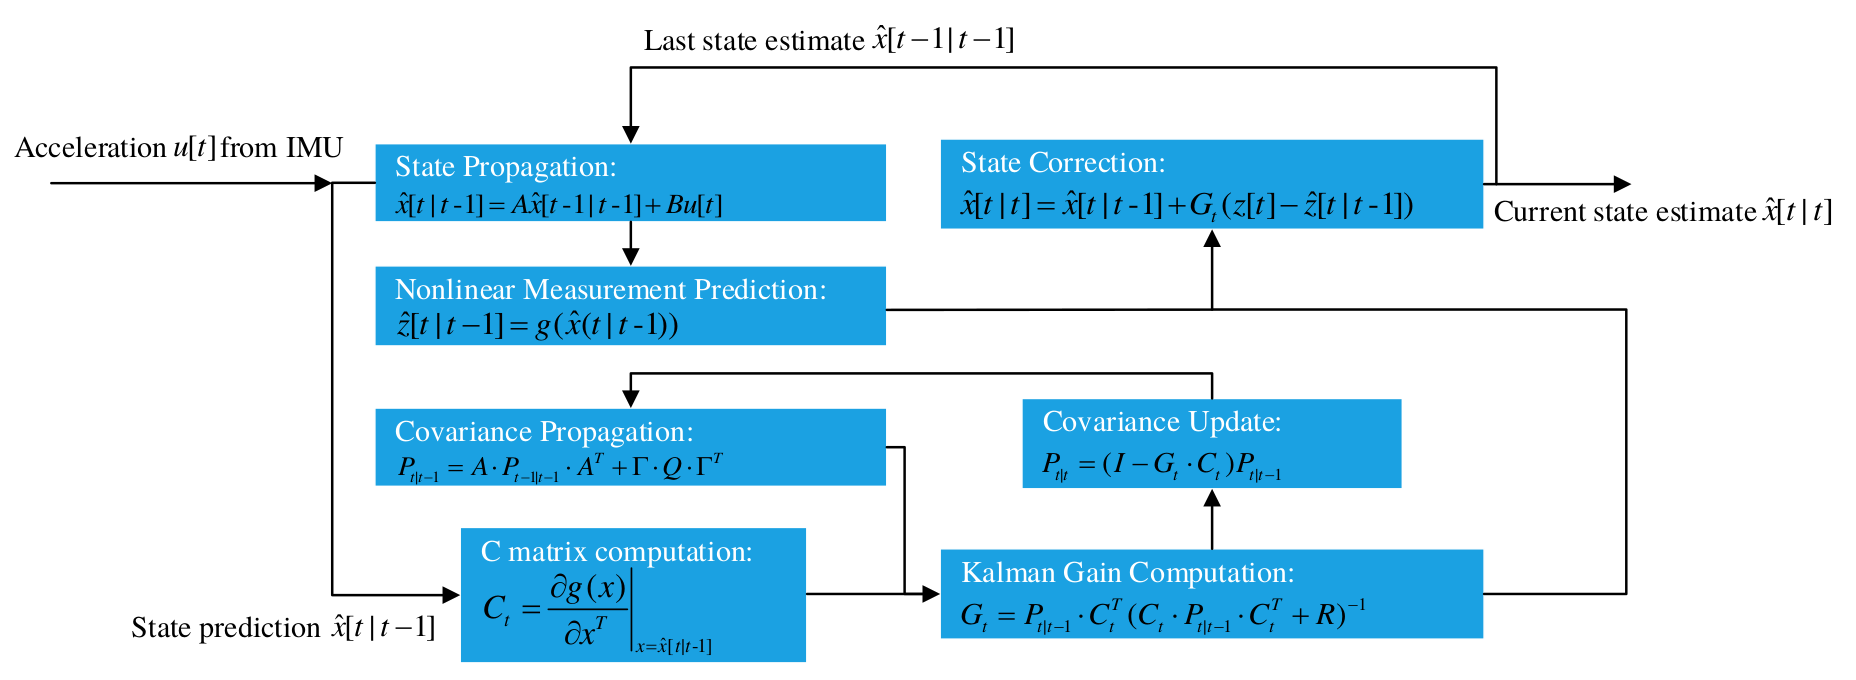
\includegraphics[width=\linewidth]{Images/Related-Work/Data-preprocessing-work-flow-using-EKF.png}
% 	\decoRule
% 	\caption[Data preprocessing work flow using EKF]{Data preprocessing work flow using EKF\cite{uwb-imu-gps1}}
% 	\label{fig:Data-preprocessing-work-flow-using-EKF}
% \end{figure}

% Ενώ σε επόμενο στάδιο, για το κομμάτι του relative position estimation, θεωρούν το σύστημα ως ένα γράφο 
% με λογική ενός \emph{spring system} - με διαφορετικούς $k_o$ συ\-ντε\-λεστές σκληρότητας - όπου στην κατάσταση 
% όπου το σύστημα σταθεροποιηθεί, θεωρείται ότι είναι το σημείο
% το οποίο περιγράφει την τοποθεσία των nodes. Ψάχνουν να βρουν το σημείο στο οποίο η συνολική δυναμική ενέργεια 
% στο σύστημα είναι η μικρότερη. Ουσιαστικά μετατρέπουν το position estimation πρόβλημα σε ένα 
% non-convex optimization πρόβλημα και προσπαθούν να το λύσουν. Ένα overview του συστήματος που δημιούργησαν 
% παρουσιάζεται στο \emph{Figure} \ref{fig:paper1-overview}.

% \begin{figure} [H]
% 	\centering
% 	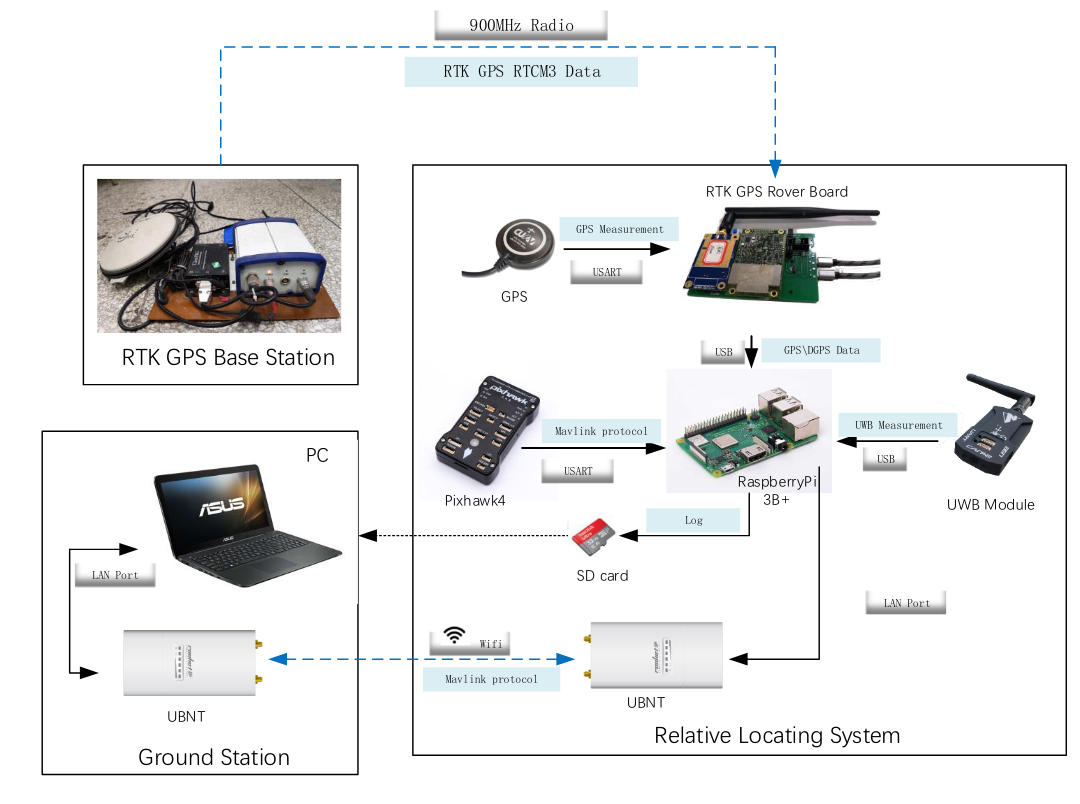
\includegraphics[width=0.69
% 	\linewidth]{Images/Related-Work/UAV-swarm-system-diagram.png}
% 	\decoRule
% 	\caption[System overview]{System overview for paper \cite{uwb-imu-gps1}}
% 	\label{fig:paper1-overview}
% \end{figure}


% ----------------------------------------------------------------





